\chapter{Use case}
\label{cha:789}
To test the operation of the previously exposed implementation, we selected an example dataset generated through a script implemented by Microsoft Azure. This choice was made due to the scarcity of online datasets that were complete enough to obtain an acceptable result. This scarcity is likely due to the sensitivity of the information contained in them.
\section{Sensor Data Generator}
The data generator is an open-source physics-inspired simulation framework that can be customised for the generation of data for model training. Generated data are a combination of telemetry and maintenance records.\\
Generated telemetry data contains:
\begin{itemize}
	\item Timestamp
	\item MachineID
	\item Ambient pressure
	\item Ambient temperature
	\item Rotational speed
	\item Desired rotational speed
	\item Temperature
	\item Pressure
\end{itemize}
Maintenance generated record contains:
\begin{itemize}
	\item Timestamp
	\item MachineID
	\item Level (INFO, WARNING, ERROR, CRITICAL)
	\item Code (identifies event/failure type)
\end{itemize}
This data does not represent a particular machinery but it is supposed that it could represent rotational motors or hydraulic pumps.\\
\section{Data Preparation}
\subsection{Data Ingestion}
In order to align the generated dataset with the data collection architecture depicted above, preliminary operations are necessary. First, a suitable structure must be created in the system. This involved the creation of a deployment, a zone, and two machines with six sensors each. Next, the generated data must be divided by sensor. This is to simulate sending the data by individual sensor. This is done by going to create records containing the timestamp, the value read from the sensor, and the sensor ID. Then, the data must be sent on the MQTT topic where the system listens. This allows the data to be uploaded to Timescale.
\subsection{Feature Engineering}
In the context of machine learning, a feature is a single measurable attribute of a physical phenomenon; the process of extracting features from raw data is called feature engineering.\\
In this case, the data is aggregated into machine cycles, which are periods of time when the machine is in a particular state; for example, the operation of an electric motor can be divided into cycles based on the states of on, rotating, and off. \\
This aggregation is necessary because the raw data cannot be used directly to train a predictive maintenance model. %Capire il perch� � necessario aggregare i dati
\\
Aggregation into cycles usually works because it is rather unlikely that there will be a sudden degradation during an operating cycle.\\
Cycles are dynamic in that they do not have a fixed duration, but adapt to the duration of the machine cycle, separating cycles when there is an interruption of at least 30 seconds in the data.\\
In addition, it is necessary to merge maintenance type data with telemetry type data aggregated by time and machine. This allows us to go in and calculate the Remaining Useful Life (RUL) based on the position of the various telemetry data in the sequence; this way we get the number of cycles for which the machine will continue to operate smoothly. For example, the cycle just before a problem will have a RUL equal to 1, the cycle before that will have a RUL equal to 2, and so on.\\ %Aggiungere data augmentation con rolling window nei future works
These operations to group the data for training were done through a complex query on Timescale, which allows us to get a data set composed in this way.
\section{Model Training}
In order to train the model, a number of preliminary operations were performed. Initially, a query was issued to the database, as previously described, and the data was then stored in Pandas data frames. These are a highly efficient two-dimensional data structure commonly used in data science. They were selected because they provide a pre-defined set of data manipulation operations and are highly efficient data structures.\\
Subsequently, sensor datasets belonging to the same machine with the same timestamp were merged into a single row, resulting in a structure that contains
\begin{itemize}
	\item asset\_id
	\item cycle
	\item speed\_desired\_max
	\item speed\_avg
	\item temperature\_avg
	\item temperature\_max
	\item pressure\_avg
	\item pressure\_max
	\item rul
\end{itemize}
Subsequently, the dataset is partitioned into two distinct data structures: "sequences" and "labels." The sequences are two-dimensional NumPy arrays that encompass all data except the rule, while the labels are NumPy arrays that exclusively contain the rule. This process results in the creation of two subdatasets, with the sequences serving as the input data for the model and the labels representing the output data that the model is tasked with predicting. The selection of a NumPy array as the data structure was driven by the necessity of aligning with the requirements of the utilised model.
\subsection{Features Scaling}
The utilisation of a deep learning model, such as LSTM, necessitates the normalisation of features. This optimises the training of the model, resulting in enhanced speed and accuracy.\\
Specifically, the normalisation of features facilitates a faster and more efficient convergence of the gradient. This, in turn, influences the training of the LSTM model, which exploits the descending vanishing problem in order to 'learn'. Furthermore, neural networks are susceptible to numerical instability issues that can be mitigated by scaling the values to eliminate those that are excessively large or small. Finally, feature normalisation enhances the model's generalisability by improving its ability to learn from diverse data.\\
In our case, we employed an object provided by the "Scikit-Learn" library called "MinMaxScaler." This object scales the data in a range from zero to one by applying a linear scaling transformation. It should be noted that this normalisation technique does not reduce the effects of outliers, as the smallest value in the dataset corresponds to 0 and the largest value in the dataset corresponds to 1.\\
The scaled values are obtained with the following formula:
\[X_{scaled} = \frac{X - X_{min}}{X_{max} - X_{min}}\]
Where X is the value that has to be scaled, $X_{min}$ is the smallest value in the dataset and $X_{max}$ is the biggest value in the dataset.
\subsection{Dataset Splitting}
The k-fold cross-validation technique was selected for training the model. The rationale behind this choice is to prevent overfitting, which occurs when a model performs well on training data but struggles with new data. The k-fold technique involves dividing the dataset into k subsets and selecting one subset for validation while the others are used for training. This process is repeated k times, with each iteration involving a different subset chosen for validation. Finally, the results of each step are averaged in order to obtain an accurate performance estimate. In this case, the "TimeSeriesSplit" object from the "scikit-learn" library was utilized to perform the split. This object enables the implementation of cross-validation, in contrast to the conventional k-fold approach, wherein the data is mixed and then split into subsets. In the case of the timeseries split, the data is split while maintaining the temporal order. The dataset is divided into consecutive subsets, with each iteration utilising data that has already been employed for training and data that is new to the model, which is then used for testing. This process is analogous to the real-world operation of training a model on historical data and then testing it on future data.
\begin{figure}[h!]
    	\centerline{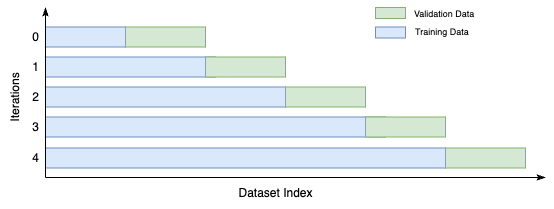
\psfig{file=timeseriessplit.png, width=0.8 \textwidth}}
\end{figure}
\subsection{Model structure}



The model comprises multiple layers, each with a distinct function. To achieve this, a sequential model from the Keras library was employed, which enables the construction of machine learning models comprising various layers. The layers utilized are as follows:
\begin{itemize}

	\item Input: This layer instructs the model regarding the size of the dataset to be passed for training.
	\item LSTM: This layer will undergo training with the LSTM model.
	\item Dropout: The dropout layer randomly sets input units to 0 with a frequency of rate at each step during training time, which helps prevent overfitting. In this case, after some trials, the chosen drop rate is 0.2.
	\item LSTM: another layer with the pattern, using two layers gives better performance in recognizing complex patterns by increasing the generalisation capabilities of the pattern. However, the problem is that having two layers makes training computationally more intensive.
	\item Dropout
	\item Batch Normalization: This process normalizes the activation of each layer by subtracting the mean and dividing by the standard deviation. It improves the training speed and helps to prevent overfitting. 
	\item Dense: this layer applies the following operation
				\[output = activation(input \cdot kernel) + bias\]
				where activation is the activation function passed as parameters, in this case "linear", kernel is a weights matrix created by the layer and bias is a vector created by the layer. It is the layer that effectively gives us an output.
\end{itemize}
Furthermore, a callback was incorporated into the model via the "EarlyStopping" object, which enables the training process to be terminated when the observed metric fails to demonstrate a continued increase. In this instance, the observed metric is the training loss, which serves to prevent overfitting. Finally, the training was conducted with a batch size of 64 and 200 epochs, resulting in a total of five repetitions of the training process, or the number of subsets created with the TimeSeriesSplit. The values in question were selected following an exhaustive series of tests designed to identify the optimal parameters, given that there is no established formula for defining them in advance.




















